
{
    The input data for visual tracking consists of a series of videos, 
    each characterized by specific and common attributes (see Table \ref{tab:video features} for the common attributes). 
    These videos form the basis for our experiments and the subsequent development of our tracking system.
}

\begin{table}[H]
    \centering
    \caption[Input videos characterization]{ \footnotesize Input video characterization }
    \label{tab:video features}

    \begin{tabularx}{0.7\textwidth}{
        @{\hspace{0.05\textwidth}}
        >{\raggedright\arraybackslash}X
        >{\raggedleft\arraybackslash}X
        @{\hspace{0.05\textwidth}}
    }
        \toprule
        \textbf{Feature Name} & \textbf{Value} \\
        \midrule
        \midrule
        Frame width & 4000 px \\
        Frame height & 2992 px \\
        Frame rate & 15 fps \\
        Color channels & Grayscale as RGB \\
        Scene type & Static \\
        Camera location & Above \\
        Encoding & MPEG4 \\
        \bottomrule
    \end{tabularx}
\end{table}

\needspace{0.1\textheight}

{
    It is important to notice that the static nature of the scenes allowed the omision of the camera motion models. 
    The frame rate of 15 fps is relatively low and it could affect the ability to roughly follow non-linear motion.
    Nevertheless, the camera location reduces the occlusions, simplifying the tracking problem. 
    The high resolution (4000x2992 px) is beneficial to experiment with the appearance models.
}

\paragraph{Video content}

{
    Our datasets consists of videos with varying content. 
    Initially, we had access to a single one-hour video containing multiple ants.
}

{
    Figure \ref{fig:full frame initial video} displays a frame from the initial video, 
    offering a view of the scene, including a zoomed-in perspective to observe a net that affected the results. 
    It is important to note that the smooth table background differs from the current one employed by the \ac{CSIC} researchers, they also stopped using the net. 
    As a result, this video was eventually replaced once additional data became available.
}

{
    The \ac{CSIC} researchers recorded 14 additional videos within two sessions.
}
 
{
    The first session included six 1-hour and six 45-minute videos. 
    The new setting featured a \textbf{hexagonal laberinth table} background, as depicted in Figure \ref{fig:frame second video}. 
    These recordings primarily served the purpose of training an appearance model and introduced several unique characteristics:
}

\begin{itemize}
    \item Each frame featured at most one ant.
    \item Whenever the \ac{CSIC} researchers introduced a new ant to the table, it was distinct from all other ants in the 12 videos.
    \item During ant exchanges, the \ac{CSIC} researchers hands briefly appears in the frame, resulting in a temporary trace of corrupted pixels.
\end{itemize}

{
    The second session contains two 1-hour videos. 
    These videos featured a tray contained multiple ants over the hexagonal laberinth table from the previous session, 
    as illustrated in Figure \ref{fig:frame third video}. 
    One of these recordings featured 87 ants, while the other contained 46 ants.
}

\begin{figure}[!p]
    \centering
    \begin{subfigure}[b]{0.4\linewidth}
        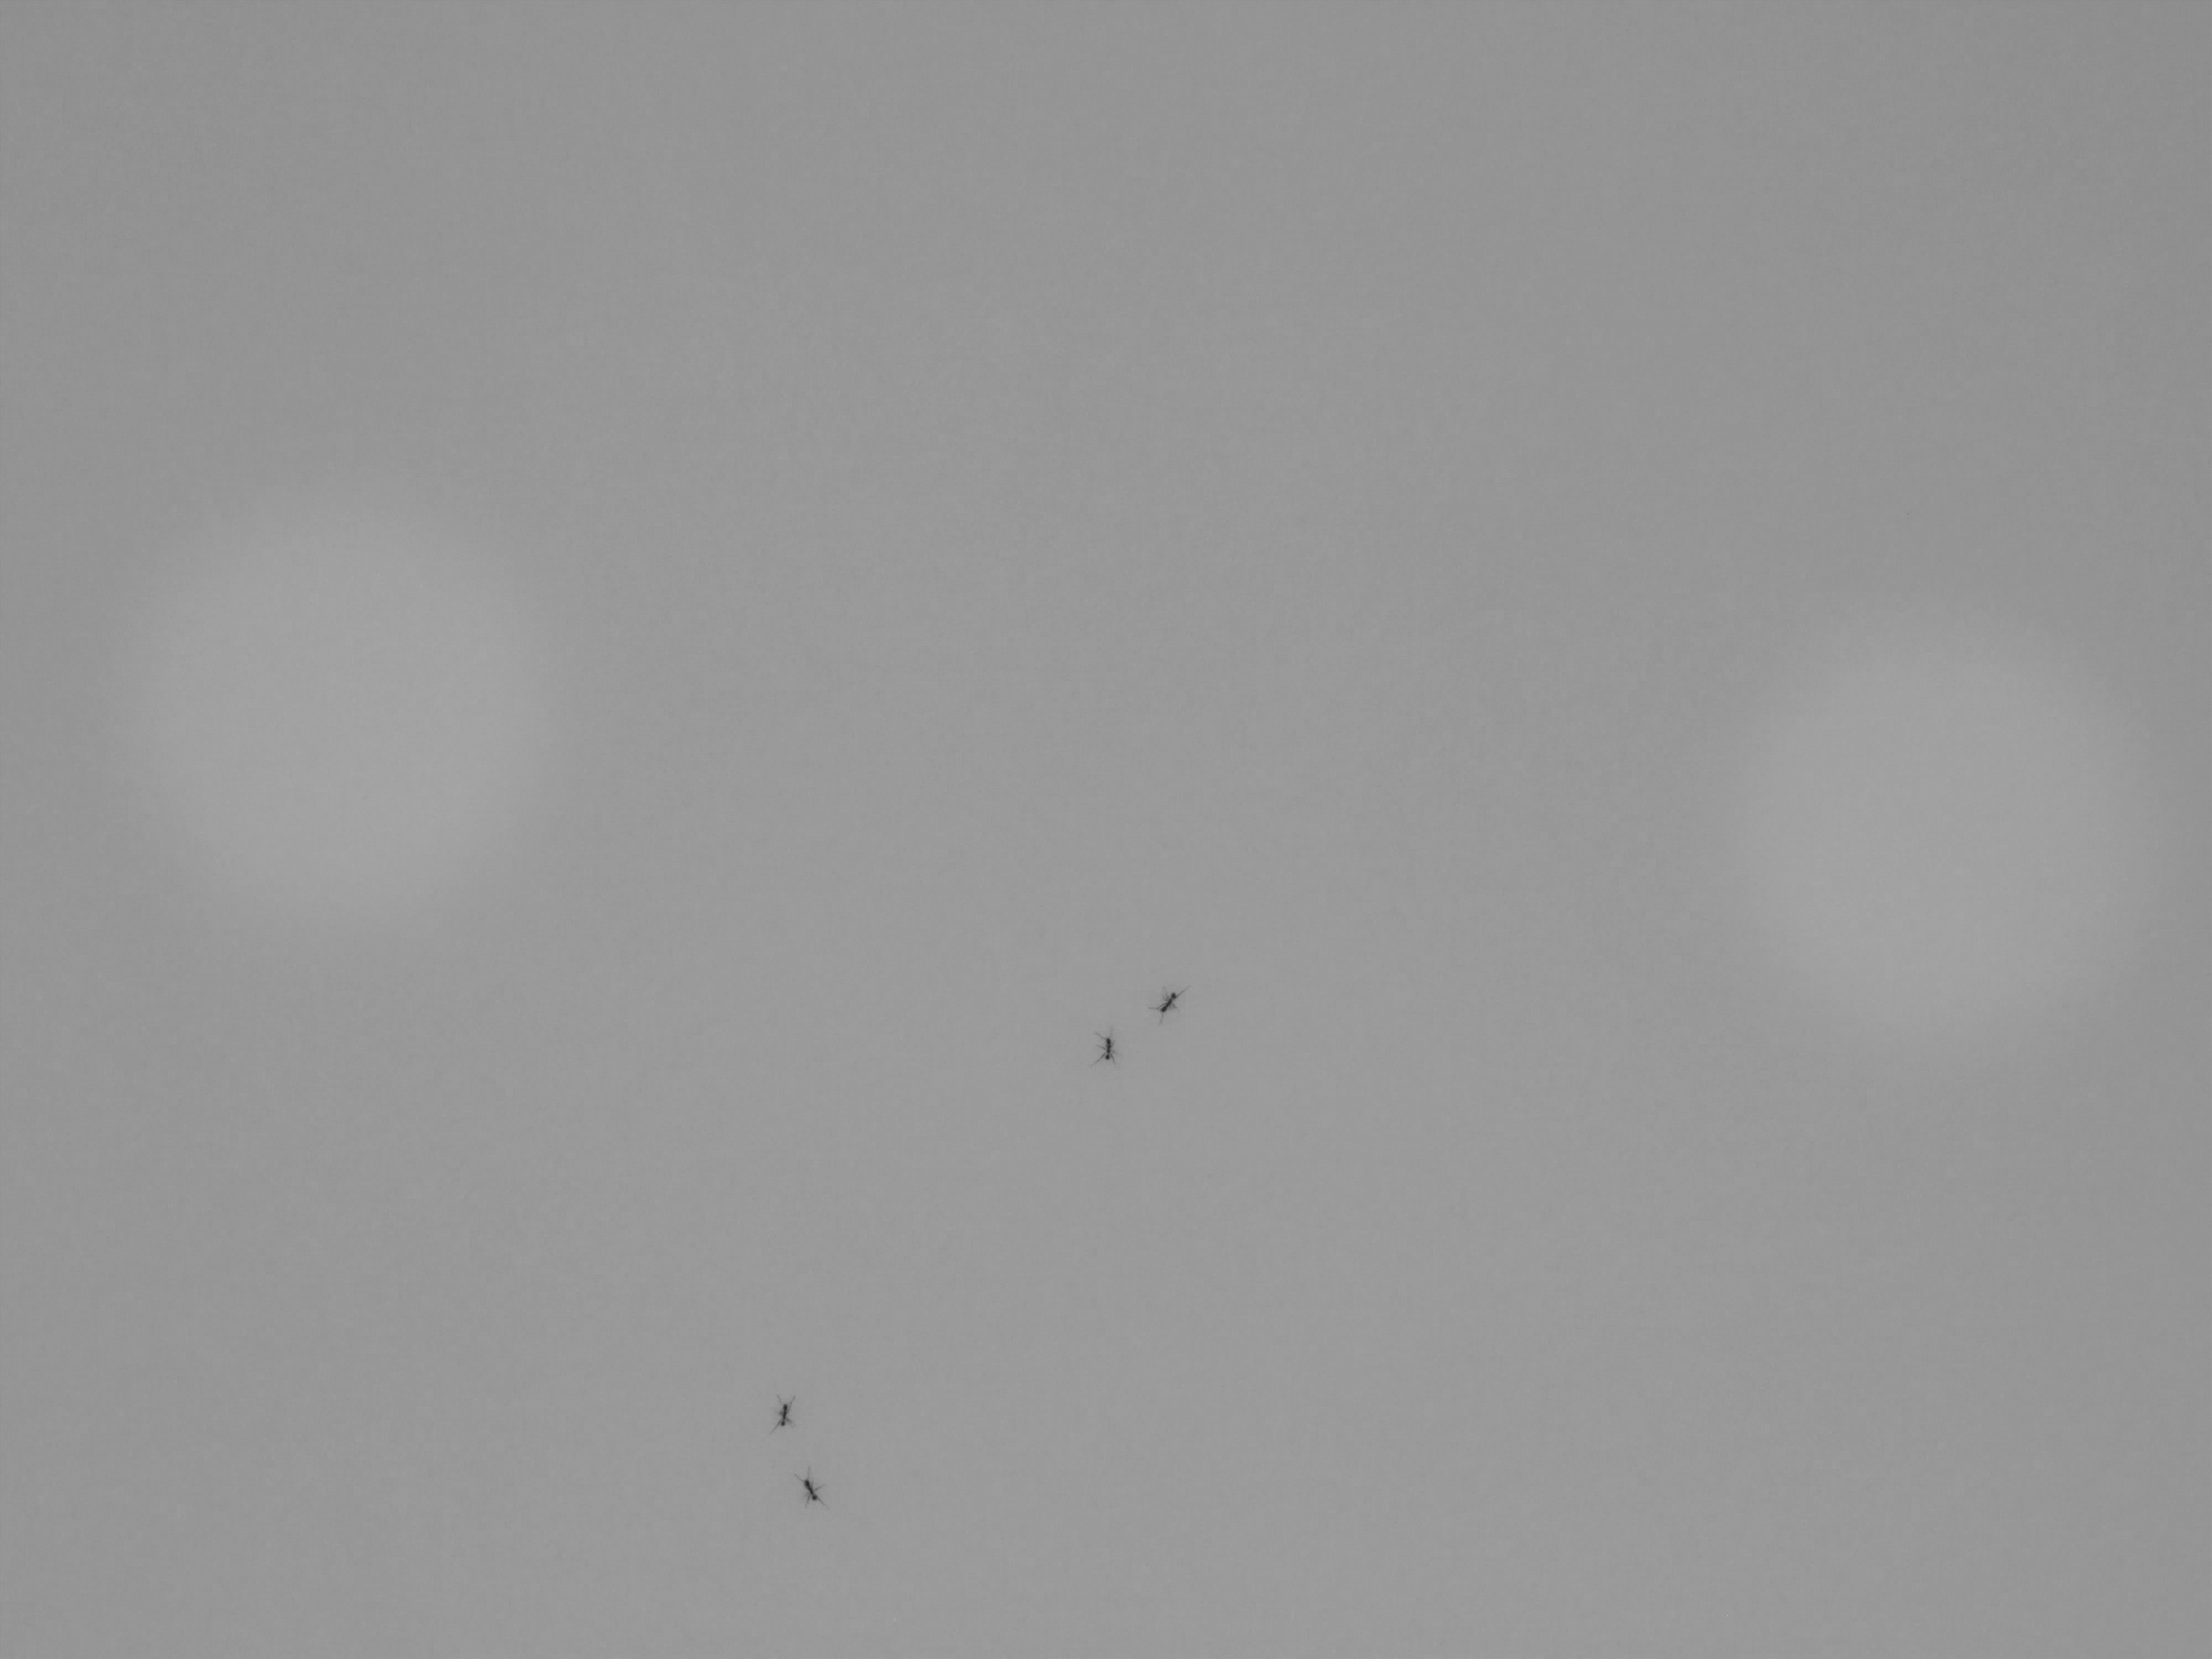
\includegraphics[width=\linewidth]{figures/05_methodology/initial_video_full.png}
        \caption[Frame from the initial video]{\footnotesize{A frame from the initial video.}}
        \label{fig:full frame initial video}
    \end{subfigure}
    \hspace{0.025\linewidth}
    \begin{subfigure}[b]{0.4\linewidth}
        \includegraphics[width=\linewidth]{figures/05_methodology/initial_video_ant.png}
        \caption[Zoom on frame from the initial video]{\footnotesize{A crop from the initial video.}}
        \label{fig:zoom frame initial video}
    \end{subfigure}
    \caption[Frame from the initial video setup]{\footnotesize{The Figure \ref{fig:zoom frame initial video} exposes the net on the upper layer of the Figure \ref{fig:full frame initial video}.}}
    \label{fig:frame initial video}
\end{figure}

\begin{figure}[!p]
    \centering
    \includegraphics[width=0.4\linewidth]{figures/05_methodology/second_video_full.png}
    \caption[Frame from the appearance video setup]{\footnotesize{A frame from one of the second set of videos.}}
    \label{fig:frame second video}
\end{figure}

\begin{figure}[!p]
    \centering
    \begin{subfigure}[b]{0.4\linewidth}
        \includegraphics[width=\linewidth]{figures/05_methodology/thirds_video_all.png}
        \caption[Frame from the more crowded tray video]{\footnotesize{A frame from the tray video with 87 ants.}}
        \label{fig:frame third video all}
    \end{subfigure}
    \hspace{0.025\linewidth}
    \begin{subfigure}[b]{0.4\linewidth}
        \includegraphics[width=\linewidth]{figures/05_methodology/thirds_video_set.png}
        \caption[Frame from the less crowded tray video]{\footnotesize{A frame from the tray video with 46 ants.}}
        \label{fig:frame third video set}
    \end{subfigure}
    \caption[Frames from the tray videos setup]{\footnotesize{Frames from the tray videos setup.}}
    \label{fig:frame third video}
\end{figure}
